%%%%%% -*- Coding: utf-8-unix; Mode: latex
% Rachunek Macierzowy — sprawozdanie, program 3.

\documentclass[polish]{template/projectreport}

\usepackage[utf8]{inputenc}
\usepackage{url}
\usepackage{indentfirst}
\usepackage{graphicx}
\usepackage{csquotes}
\DeclareQuoteStyle[quotes]{polish}
  {\quotedblbase}
  {\textquotedblright}
  [0.05em]
  {\quotesinglbase}
  {\fixligatures\textquoteright}
\DeclareQuoteAlias[quotes]{polish}{polish}

\graphicspath{{figures/}}

\usepackage{xcolor}
\usepackage{listings}
\usepackage{booktabs}
\usepackage{amsmath}

\definecolor{codegreen}{rgb}{0,0.5,0}
\lstdefinestyle{matlab}{
  language=Matlab,
  basicstyle=\ttfamily\footnotesize,
  keywordstyle=\color{blue}\bfseries,
  commentstyle=\color{codegreen},
  breaklines=true,
  frame=single,
  numbers=left,
  numberstyle=\tiny\sffamily,
  tabsize=2,
  showstringspaces=false
}
\lstset{style=matlab}
\AtBeginDocument{%
  \shorthandoff{"}%
  \addto\captionspolish{\renewcommand{\lstlistingname}{Fragment kodu}}%
}

\usepackage[bookmarks=false]{hyperref}
\hypersetup{colorlinks,
  linkcolor=blue,
  citecolor=blue,
  urlcolor=blue}

\newcommand{\TytulZadania}{Normy macierzowe, uwarunkowanie i~rozkład SVD}
\newcommand{\NumerProgramu}{3}
\newcommand{\Autorzy}{Kacper Bujak, Wojciech Maćkowiak}

\title{\TytulZadania\\{\large Rachunek Macierzowy --- program \NumerProgramu}}
\author{\Autorzy}
\date{\today}

\begin{document}
% auto-generated przez solution.m
\newcommand{\ValNOne}{2.061568e+01}
\newcommand{\ValNTwo}{1.645829e+01}
\newcommand{\ValNInf}{2.052300e+01}
\newcommand{\ValNSchat}{1.648238e+01}
\newcommand{\ValCOne}{2.296702e+03}
\newcommand{\ValCTwo}{9.052938e+02}
\newcommand{\ValCInf}{2.205520e+03}
\newcommand{\ValCSchat}{9.069105e+02}
\newcommand{\ValSigmaMin}{1.818006e-02}
\newcommand{\ValSigmaMax}{1.645829e+01}
\newcommand{\ValSVDRes}{5.532555e-14}
\newcommand{\ValRcond}{4.354069e-04}
\newcommand{\ValEigRes}{3.625770e-14}
\newcommand{\ValCOneDef}{2.296702e+03}
\newcommand{\ValCTwoDef}{9.052938e+02}
\newcommand{\ValCInfDef}{2.205520e+03}
\newcommand{\ValBuiltinNOne}{2.061568e+01}
\newcommand{\ValBuiltinNTwo}{1.645829e+01}
\newcommand{\ValBuiltinNInf}{2.052300e+01}
\newcommand{\ValBuiltinCOne}{2.296702e+03}
\newcommand{\ValBuiltinCTwo}{9.052938e+02}
\newcommand{\ValBuiltinCInf}{2.205520e+03}
\newcommand{\ValBuiltinNSchat}{1.648238e+01}
\newcommand{\ValBuiltinKSchat}{9.069105e+02}
\newcommand{\ValAbsDiffNOne}{0.000000e+00}
\newcommand{\ValAbsDiffNTwo}{0.000000e+00}
\newcommand{\ValAbsDiffNInf}{0.000000e+00}
\newcommand{\ValAbsDiffCOne}{0.000000e+00}
\newcommand{\ValAbsDiffCTwo}{0.000000e+00}
\newcommand{\ValAbsDiffCInf}{0.000000e+00}
\newcommand{\ValAbsDiffNSchat}{3.552714e-15}
\newcommand{\ValAbsDiffKSchat}{1.136868e-13}
\newcommand{\ValRelDiffNOne}{0.000000e+00}
\newcommand{\ValRelDiffNTwo}{0.000000e+00}
\newcommand{\ValRelDiffNInf}{0.000000e+00}
\newcommand{\ValRelDiffCOne}{0.000000e+00}
\newcommand{\ValRelDiffCTwo}{0.000000e+00}
\newcommand{\ValRelDiffCInf}{0.000000e+00}
\newcommand{\ValRelDiffNSchat}{2.155462e-16}
\newcommand{\ValRelDiffKSchat}{1.253562e-16}


\maketitle

\section{Cel ćwiczenia}
Dla kwadratowej macierzy rzeczywistej $M$ obliczyć normy macierzowe $\|M\|_1$, $\|M\|_2$, $\|M\|_\infty$, normę z~klasy norm Schattena dla ustalonego rzędu~$p$ (wartości osobliwe z~SVD), odpowiadające współczynniki uwarunkowania, pełny rozkład SVD oraz wartości i~wektory własne przy użyciu procedur numerycznych Octave (\texttt{svd}, \texttt{eig}); normy indukowane i~\texttt{cond} zaimplementowano samodzielnie i~zweryfikowano względem wbudowanych \texttt{norm} i~\texttt{cond}.

Macierz testowa: losowa $n\times n$ przy $n = 8 + 24 = 32$ (jak w~programie~2), ziarno generatora \texttt{rng(11)}, odrzucenie macierzy z~$\texttt{rcond}(M)$ zbyt małym.

\section{Opis metody / algorytmu}

\subsection{Norma $\|M\|_1$ i~$\|M\|_\infty$}
Norma indukowana z~normy wektorowej ``suma modułów'': $\|M\|_1 = \max_j \sum_i |M_{ij}|$ (największa suma modułów po kolumnach). Norma $\|M\|_\infty = \max_i \sum_j |M_{ij}|$ --- po wierszach.

\subsection{Norma $\|M\|_2$}
$\|M\|_2 = \sigma_{\max}(M)$ --- największa wartość osobliwa (spektralna norma operatora liniowego w~parze norm euklidesowych na $\mathbb{R}^n$).

\subsection{Norma Schattena $\|M\|_{S,p}$ dla ustalonego $p$}
Niech $\sigma_1 \ge \cdots \ge \sigma_n \ge 0$ będą wartościami osobliwymi $M$. Norma Schattena rzędu~$p$ (dla macierzy rzeczywistej): $\|M\|_{S,p} = \bigl(\sum_i \sigma_i^p\bigr)^{1/p}$. Dla $p=2$ pokrywa się z~normą Frobeniusa $\|M\|_F$, a~nie z~$\|M\|_2$; w~niniejszym zadaniu przyjęto $p=4$, by wypełnić punkt ``$\|M\|_p$'' w~sposób jednoznaczny i~powiązany z~SVD.

\subsection{Współczynnik uwarunkowania}
Dla norm indukowanych $1$, $2$, $\infty$: $\kappa(M) = \|M\|\,\|M^{-1}\|$. Octave zwraca to przez \texttt{cond(M,1)}, \texttt{cond(M)} (dla~$2$), \texttt{cond(M,inf)}. Dla normy Schattena przyjmujemy analogicznie $\kappa_{S,p} = \|M\|_{S,p}\,\|M^{-1}\|_{S,p}$; wartości osobliwe $M^{-1}$ to $1/\sigma_i$, stąd $\|M^{-1}\|_{S,p} = \bigl(\sum_i \sigma_i^{-p}\bigr)^{1/p}$.

\subsection{SVD i~wartości własne}
Rozkład $M = U \Sigma V^{\mathsf T}$ z~$\Sigma$ diagonalną nieujemną. Rozkład spektralny (wartości własne, wektory w~kolumnach macierzy $V$) daje \texttt{eig(M)} dla macierzy rzeczywistej (wartości własne mogą być zespolone).

\section{Implementacja}
W~katalogu \texttt{src/}: skrypt \texttt{solution.m} ustala $M$, liczy normy i~uwarunkowanie własnymi funkcjami, \textbf{porównuje} wyniki z~wbudowanymi \texttt{norm}/\texttt{cond} (oraz \texttt{norm} na wektorze~$\sigma$ dla Schattena), wywołuje \texttt{inv} do weryfikacji definicji $\|M\|\,\|M^{-1}\|$, \texttt{svd}, \texttt{eig}, oraz \texttt{schatten\_norm\_cond.m}. Wyniki liczbowe do tabel zapisuje się do \texttt{wyniki\_auto.tex}; do wykresów w~Pythonie: \texttt{singular\_values.txt}, \texttt{norms\_bar.txt}, \texttt{cond\_samples.txt} (ostatni z~proby $250$ losowych macierzy $n\times n$ o~rozsądnym \texttt{rcond}). Skrypt \texttt{analysis/plot\_template.py} generuje kilka plików PDF w~\texttt{LaTeX/figures/}.

\section{Fragmenty kodu}

\subsection{Norma wektorowa \texttt{l\_p} (\texttt{vector\_norm\_p.m})}
\lstinputlisting{../src/vector_norm_p.m}

\noindent\texttt{x(:)} --- wektor w~jednej kolumnie.\\
\texttt{isinf(p)\&\&p>0}: norma $\|x\|_\infty=\max_i|x_i|$.\\
\texttt{else}: $\|x\|_p=\bigl(\sum_i|x_i|^p\bigr)^{1/p}$.\\

\subsection{Normy macierzowe indukowane $1$, $2$, $\infty$ (\texttt{matrix\_norm\_induced.m})}
\lstinputlisting{../src/matrix_norm_induced.m}

\noindent $p=1$: $\|M\|_1=\max_j\sum_i|M_{ij}|$ --- największa suma modułów po kolumnach (\texttt{sum(...,1)} i~\texttt{max}).\\
$p=\infty$ (test \texttt{isinf(p)}): $\|M\|_\infty=\max_i\sum_j|M_{ij}|$ --- po wierszach (\texttt{sum(...,2)})\\
$p=2$: spektralna norma $\|M\|_2=\sigma_{\max}(M)$ jako \texttt{max(svd(M))}.\\

\subsection{Norma Frobeniusa (\texttt{matrix\_norm\_fro.m})}
\lstinputlisting{../src/matrix_norm_fro.m}

\noindent $\|M\|_F=\bigl(\sum_{i,j}|m_{ij}|^2\bigr)^{1/2}$

\subsection{Uwarunkowanie w~normach indukowanych (\texttt{matrix\_cond\_induced.m})}
\lstinputlisting{../src/matrix_cond_induced.m}

\noindent $\kappa_p(M)=\|M\|_p\,\|M^{-1}\|_p$ w~normie indukowanej (pełny rząd).\\

\subsection{Norma Schattena i~$\kappa_{S,p}$ (\texttt{schatten\_norm\_cond.m})}
\lstinputlisting{../src/schatten_norm_cond.m}

\noindent Argument \texttt{s} to wektor wartości osobliwych (wynik \texttt{svd(M)}).\\
\texttt{nrm} to $\|s\|_p$, czyli norma Schattena $\|M\|_{S,p}$.\\
Gdy któreś $s\le 0$: $\kappa=\infty$ (brak odwrotności w~pełnym sensie).\\
Inaczej $\kappa=\|s\|_p\,\|v\|_p$ przy $v_i=\sigma_i^{-1}$ (w~kodzie odwrotności element po elemencie).\\
Norma na wektorze liczy \texttt{vector\_norm\_p}.


\section{Wyniki numeryczne}

\subsection{Normy i~uwarunkowanie}
\begin{table}[htbp]
  \centering
  \caption{Normy macierzy $M$ i~współczynniki uwarunkowania (wartości z~uruchomienia \texttt{solution.m}).}
  \begin{tabular}{@{}l r@{}}
    \toprule
    Wielkość & Wartość \\
    \midrule
    $\|M\|_1$ & \ValNOne \\
    $\|M\|_2$ & \ValNTwo \\
    $\|M\|_\infty$ & \ValNInf \\
    $\|M\|_{S,4}$ (Schatten) & \ValNSchat \\
    \midrule
    $\texttt{cond}(M,1)$ & \ValCOne \\
    $\|M\|_1 \|M^{-1}\|_1$ & \ValCOneDef \\
    $\texttt{cond}(M,2)$ & \ValCTwo \\
    $\|M\|_2 \|M^{-1}\|_2$ & \ValCTwoDef \\
    $\texttt{cond}(M,\infty)$ & \ValCInf \\
    $\|M\|_\infty \|M^{-1}\|_\infty$ & \ValCInfDef \\
    $\kappa_{S,4}$ & \ValCSchat \\
    \bottomrule
  \end{tabular}
\end{table}

\begin{table}[htbp]
  \centering
  \footnotesize
  \caption{Porównanie własnej implementacji z~wbudowanymi \texttt{norm} / \texttt{cond} w~Octave (ta sama macierz $M$). Dla $\|M\|_{S,4}$ i~$\kappa_{S,4}$ w~kolumnie ,,Octave'' podano odpowiednio \texttt{norm(s(:),4)} oraz iloczyn \texttt{norm(s(:),4)*norm(1./s(:),4)} na wektorze wartości osobliwych \texttt{s = svd(M)} (brak macierzowego \texttt{cond} dla normy Schattena). Kolumna ,,wzgl.'' to $|\Delta|/\max(|\text{Octave}|,\varepsilon)$.}
  \begin{tabular}{@{}l r r r r@{}}
    \toprule
    Wielkość & własna & Octave & $|\Delta|$ & wzgl. \\
    \midrule
    $\|M\|_1$ & \ValNOne & \ValBuiltinNOne & \ValAbsDiffNOne & \ValRelDiffNOne \\
    $\|M\|_2$ & \ValNTwo & \ValBuiltinNTwo & \ValAbsDiffNTwo & \ValRelDiffNTwo \\
    $\|M\|_\infty$ & \ValNInf & \ValBuiltinNInf & \ValAbsDiffNInf & \ValRelDiffNInf \\
    $\texttt{cond}(M,1)$ & \ValCOne & \ValBuiltinCOne & \ValAbsDiffCOne & \ValRelDiffCOne \\
    $\texttt{cond}(M,2)$ & \ValCTwo & \ValBuiltinCTwo & \ValAbsDiffCTwo & \ValRelDiffCTwo \\
    $\texttt{cond}(M,\infty)$ & \ValCInf & \ValBuiltinCInf & \ValAbsDiffCInf & \ValRelDiffCInf \\
    $\|M\|_{S,4}$ & \ValNSchat & \ValBuiltinNSchat & \ValAbsDiffNSchat & \ValRelDiffNSchat \\
    $\kappa_{S,4}$ & \ValCSchat & \ValBuiltinKSchat & \ValAbsDiffKSchat & \ValRelDiffKSchat \\
    \bottomrule
  \end{tabular}
\end{table}

Wiersze z~definicją $\|M\|\,\|M^{-1}\|$ pokrywają się z~wyjściem \texttt{cond} --- zgodnie z~teorią dla norm indukowanych.

Małe residuum rozkładu SVD oraz residuum $M V = V D$ potwierdzają poprawność obliczeń bibliotecznych.

\subsection{Wykresy}

Spektrum wartości osobliwych (rys.~\ref{fig:sigma}) pokazuje szybki spadek $\sigma_i$: typowe dla losowej macierzy pełnej --- energia Frobeniusa koncentruje się na kilku dominujących kierunkach. Rysunek~\ref{fig:energia} formalizuje to jako skumulowany udział $\sum_{i\le k}\sigma_i^2 / \|M\|_F^2$: często wystarczy niewiele składowych, by przekroczyć np.\ $90\%$ tej energii.

\begin{figure}[htbp]
  \centering
  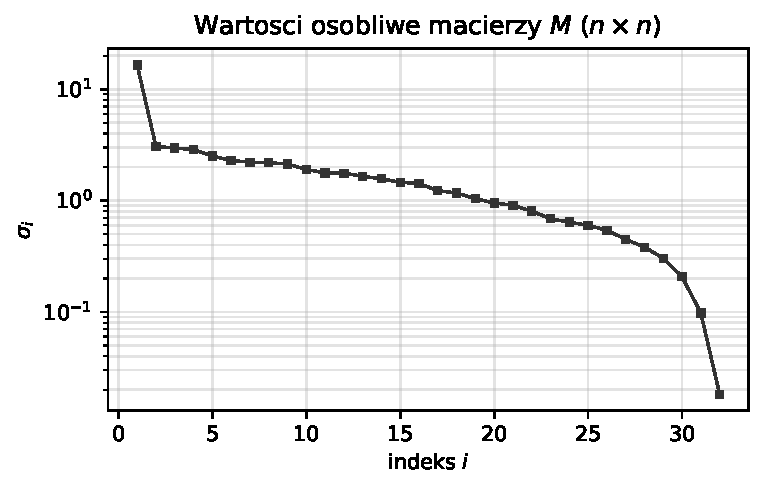
\includegraphics[width=0.72\linewidth]{wartosci_osobliwe.pdf}
  \caption{Wartości osobliwe $\sigma_i$ macierzy $M$ (oś $y$ w~skali logarytmicznej).}
  \label{fig:sigma}
\end{figure}

\begin{figure}[htbp]
  \centering
  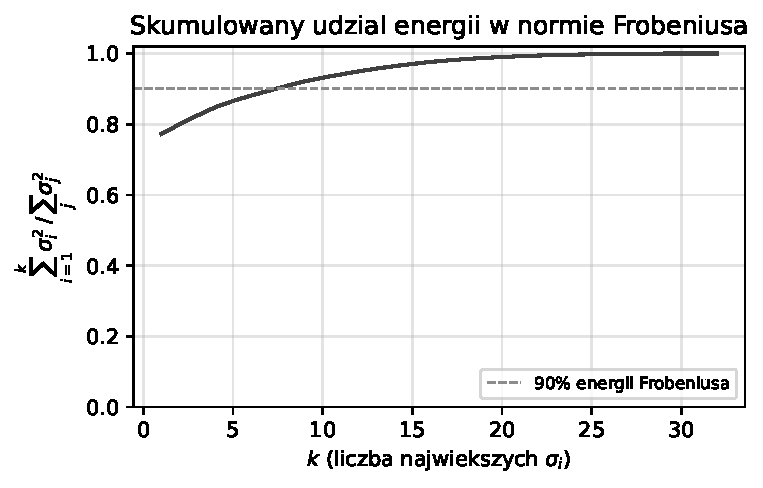
\includegraphics[width=0.72\linewidth]{energia_frobeniusa_skumulowana.pdf}
  \caption{Skumulowany udział $\|M\|_F^2$ w~największych wartościach osobliwych (rank-$k$ przybliżenie w~normie Frobeniusa).}
  \label{fig:energia}
\end{figure}

Na rys.~\ref{fig:normy} widać, że dla tej samej macierzy $M$ normy indukowane $1$, $2$, $\infty$ oraz norma Schattena $S{,}4$ nie muszą być równe: są to różne sposoby mierzenia ``rozmiaru'' operatora; nierówności teoretyczne (np.\ $\|M\|_2 \le \|M\|_F$) można sprawdzić liczbowo na tabeli z~sekcji wcześniejszej.

\begin{figure}[htbp]
  \centering
  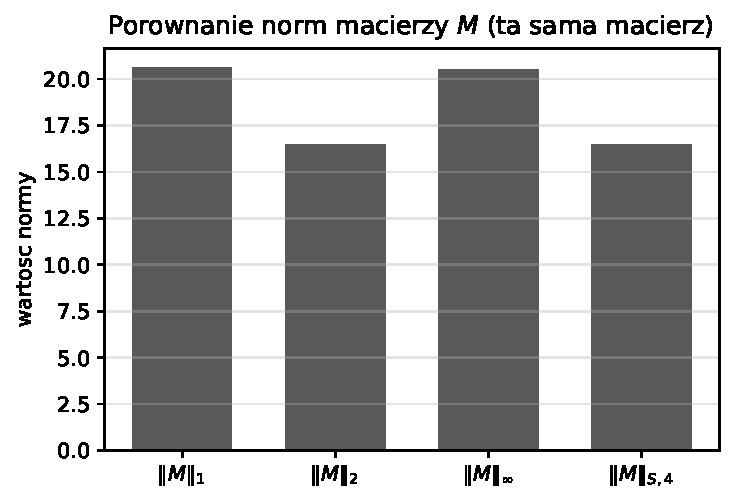
\includegraphics[width=0.65\linewidth]{normy_porownanie.pdf}
  \caption{Porównanie czterech norm dla jednej macierzy testowej $M$.}
  \label{fig:normy}
\end{figure}

Rysunek~\ref{fig:cond} przedstawia empiryczny rozkład $\texttt{cond}(A,2)$ dla wielu losowych $A$ o~tym samym $n$ co $M$. Rozkład jest silnie prawoskośny w~skali logarytmicznej: większość macierzy ma umiarkowane uwarunkowanie, a~``ogony'' odpowiadają rzadkim, trudniejszym numerycznie realizacjom --- stąd sens sprawdzania \texttt{rcond} przed obliczeniami na odwróconej macierzy.

\begin{figure}[htbp]
  \centering
  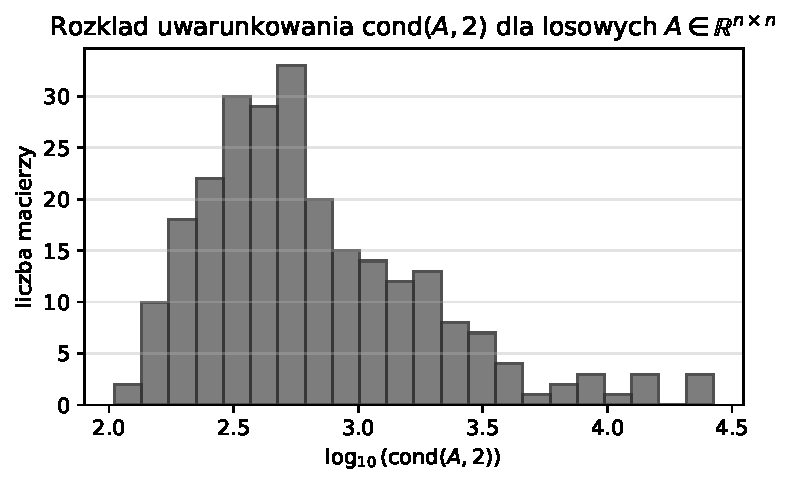
\includegraphics[width=0.72\linewidth]{rozklad_cond2_losowe.pdf}
  \caption{Histogram $\log_{10}(\texttt{cond}(A,2))$ dla losowych macierzy $A\in\mathbb{R}^{n\times n}$ ($n=32$, odfiltrowane osobliwe / złe \texttt{rcond}).}
  \label{fig:cond}
\end{figure}

\section{Wnioski}

\begin{itemize}
  \item \textbf{Zgodność z~Octave i~definicją.} Własne funkcje dają te same wartości co wbudowane \texttt{norm} i~\texttt{cond} dla norm indukowanych $1$, $2$, $\infty$ (różnice na poziomie zera maszynowego); norma Schattena i~$\kappa_{S,4}$ zgadzają się z~\texttt{norm} na wektorze~$\sigma$ z~dokładnością rzędu $10^{-15}$--$10^{-13}$. Jednocześnie $\texttt{cond}(M,\cdot)$ pokrywa się z~iloczynem $\|M\|\,\|M^{-1}\|$ w~tej samej normie.
  \item \textbf{Różne normy, różna geometria.} Normy indukowane mierzą maksymalne wzmocnienie wektora w~innych normach wektorowych; norma Schattena $S{,}4$ zależy od całego spektrum singularnego i~dla $p\neq 2$ nie pokrywa się z~$\|M\|_2$. W~raporcie przyjęto $p=4$ świadomie, by powiązać punkt ``$\|M\|_p$'' z~SVD i~uniknąć niejednoznaczności ogólnej normy indukowanej $\|\cdot\|_p$ dla macierzy.
  \item \textbf{SVD a stabilność.} Bardzo małe residuum $\|M-U\Sigma V^{\mathsf T}\|_F$ pokazuje, że numeryczny SVD jest stabilny dla naszej macierzy; stosunek $\sigma_{\max}/\sigma_{\min}$ kontroluje $\texttt{cond}(M,2)$ i~wrażliwość na błędy zaokrągleń przy rozwiązywaniu układów z~$M$.
  \item \textbf{Wartości własne vs osobliwe.} Dla macierzy niesymetrycznej moduły wartości własnych nie muszą pokrywać się z~$\sigma_i$; widoczna zespoloność $\lambda$ przy rzeczywistym $M$ jest normalna. Małe residuum spektralne $\|MV-VD\|_F$ świadczy o~poprawnym zestawieniu par własnych z~\texttt{eig}.
  \item \textbf{Losowe macierze a typowe uwarunkowanie.} Histogram $\texttt{cond}(A,2)$ sugeruje, że ``typowa'' losowa macierz ma uwarunkowanie znacznie mniejsze niż pesymistyczne szacunki teoretyczne dla najgorszego przypadku; jednocześnie ogon rozkładu przypomina, że przy wielu losowaniach warto odrzucać patologiczne $A$ (tutaj przez próg na \texttt{rcond}).
  \item \textbf{Energia w~SVD.} Krzywa skumulowanej energii Frobeniusa wskazuje, że niskorzędowe przybliżenie $M$ może być dokładne w~normie Frobeniusa nawet przy małym $k$ --- intuicja przydatna przy PCA / kompresji danych i~analizie skutecznego wymiaru operatora.
\end{itemize}

\end{document}
